\chapter{Data preparation process}
This chapter describes the process of preparing the data.

%\section{Data analysis} kanske ha denna sen
	%explain the process of analyzing the data

\section{Data cleaning} \label{sec:datacleaning}
	 In the provided guidelines (see \ref{sec:provided_data}), there is a note on the measurements from station 1429 saying: "Unreasonable DST111 measurements from about 2016-11-15 to 2016-12-31". It was found in the measurements from the 1429 that the average difference between the DST111 and Track Ice Road Surface road surface temperature measurements were $~1.71 \celsius$ whereas in stations 1402 and 1431, which are the two geographically closest stations to 1429, the average differences were $0.614 \celsius$ and  $~0.54 \celsius$. In some cases, the difference between the measurements from the two temperature sensors in station 1429 were above $40 \celsius$. This indicates that something may have been wrong with DST111, or some other instrument at the time and thus, the observations from 2016-11-15 to 2016-12-31 were removed from the workbook containing data from station 1429. This resulted in an average road surface temperature difference of $~0.92 \celsius$, which is higher still than the two nearby stations, but whether this was unreasonable or not could not be determined by the author. 

	In addition to removing suspicious outliers in the dataset, there are also cases where errors are explicitly reported by the sensors. As mentioned in \ref{sec:delimitations}, only non-error features are used in this project. As of such, every observation where at least one error is reported by any sensor, are removed. Figure \ref{img:histogram_surfstatus} shows that the DSC111 alone was malfunctioning for unknown reasons in more than $50 000$ observations. 

\begin{figure}[H] 
	\centering
	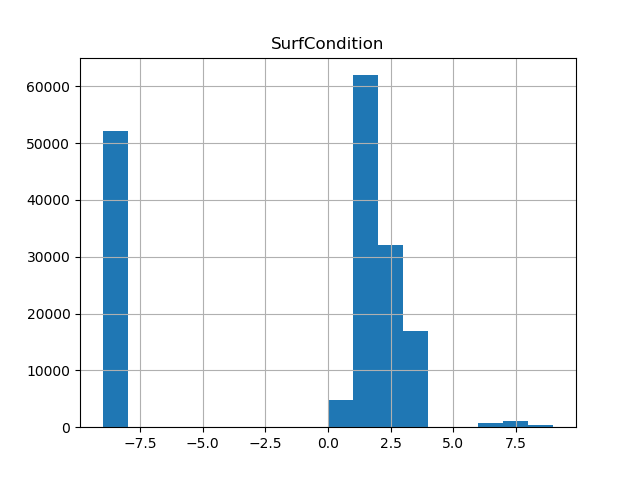
\includegraphics[width=0.8\textwidth]{media/HistogramSurfaceStatus.png}
	\caption{Histogram showing the distribution of the different surface status types (see \ref{table:discretevalues} to see what each code means).}
	\label{img:histogram_surfstatus}
\end{figure}

	More suspicious outliers may be present in the dataset that could potentially be identified by applying, for example, a confidence interval. But it was decided to not investigate this matter further since it was assumed that analytical knowledge in road condition data is needed to decide if an outlier represents an error or a correct abnormal value. After the data cleaning process, a total of 115180 observations remained, which means 56245 observations were removed.


\section{Feature selection}
	It was decided to investigate if time should be excluded as a possible input feature, primarily because the values it presents are higher than the rest of the features. Some supervised learning algorithms, such as kNN, are sensitive to scaling (see \ref{sec:knn}). Time is interpreted as integers by any model that use it as an input feature. For example, an observation from station 1520 from 12/31/2016 23:30 have the following values: $\text{time} = 12312330, \text{SurfTemp }= 7.1, ... \text{Friction} = 0.74$. 

	Although the scaling of the time feature is significantly different from the other input features, it seems to be correlated with other features. Figure \ref{img:correlations_noerr} shows how every feature is related to one another, it indicates that features such as time and friction are correlated with time. The correlation may come as no surprise since the northern hemisphere is colder during winter-time, which means cold temperatures and low friction, and the other way around during warmer periods. 

\begin{figure}[H] 
	\centering
	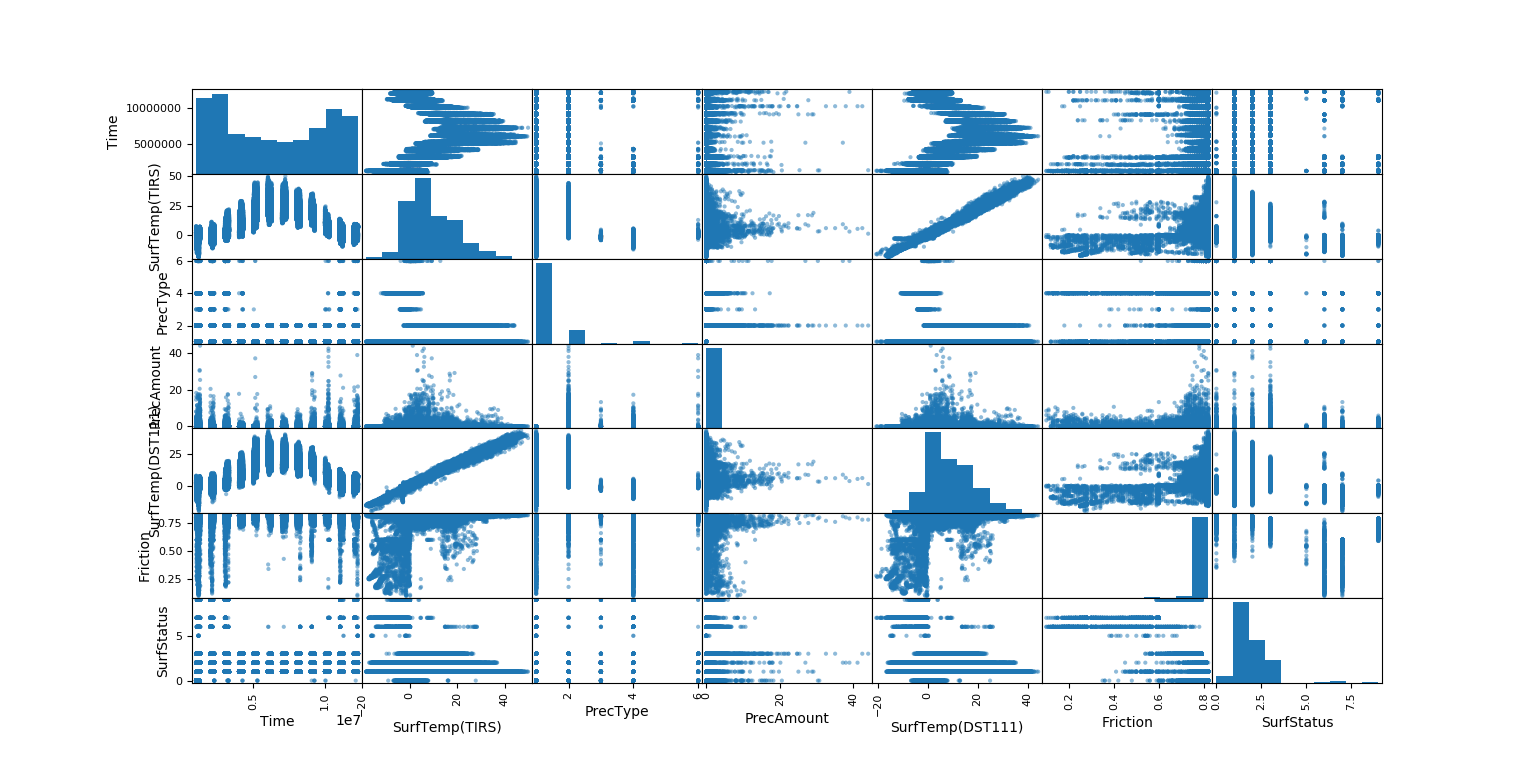
\includegraphics[width=1\textwidth]{media/relationship_parameters_pre_noerr.png}
	\caption{Depicts how the features are correlated to oneanother.}
	\label{img:correlations_noerr}
\end{figure}

	To test the relevance of using time as input feature, an experiment was carried out to predict Track Ice Road Sensor road surface temperature once with time as input feature, and once without. The experiment runs the Cross-validation regression spot-checking setup (see \ref{sec:exp_setups}). Table \ref{table:timeinput} shows the result from the experiment.

	\begin{table}[H] %gör om med holdout
	\centering
	\caption{Experiment to see if time is relevant to use as input feature. }
		\begin{tabular}[3]{l | c | c}
    			Algorithm & MSE not using time & MSE using time \\
    			\hline
			OLS & 1.23 & 1.22 \\
			CART & 1.21 & 1.84 \\
			kNN & 1.25 & 4.69 \\
			Backpropagation & 1.06 & 769096.72 \\
			Lasso & 1.25 & 1.24 \\
			Random forest & 1.13 & 1.26 \\
			\hline
			Average total & 1.19 & 128184.50
			\label{table:timeinput}
		\end{tabular}
	\end{table}

	The results indicate that OLS, Lasso and Random forest achieve slightly better performance by using time as input feature, whereas CART, kNN, Random forest and especially Backpropagation, suffer in terms of performance when doing so. This is an indication that overall performance is improved by not using time as input feature, but the possibility of using this data is not ruled out yet. Section \ref{sec:transformation} deals with testing if time can be scaled down to similar levels of other features to see if it improves overall performance or not.

\section{Data transformation} \label{sec:transformation}

	\subsection{Rescaling time}

	Table \ref{table:timeinput} shows significant improvement in overall performance in not using time as input feature. However,  \ref{img:correlations_noerr} shows that time may be a relevant feature to include in that it shows correlation with other features. It was decided to test if a transformation of the time feature could yield better performance than using it in its original form. The transformation involves using only month, and time of day from the time feature but to separate it into two columns so that they operate on lower numeric intervals than combining them. Figure \ref{img:transformation} shows the transformation. 

\begin{figure}[H] 
	\centering
	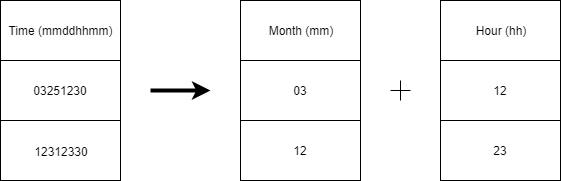
\includegraphics[width=0.8\textwidth]{media/transformation_time.png}
	\caption{Shows how time as feature is transformed to two new features: month and hour.}
	\label{img:transformation}
\end{figure}

	The author assumes that month and time of day affect changes in weather conditions more than separate days within a month. Figure \ref{img:correlations_featureengi} shows the correlations among the features with month and hour used instead of time. 

\begin{figure}[H] 
	\centering
	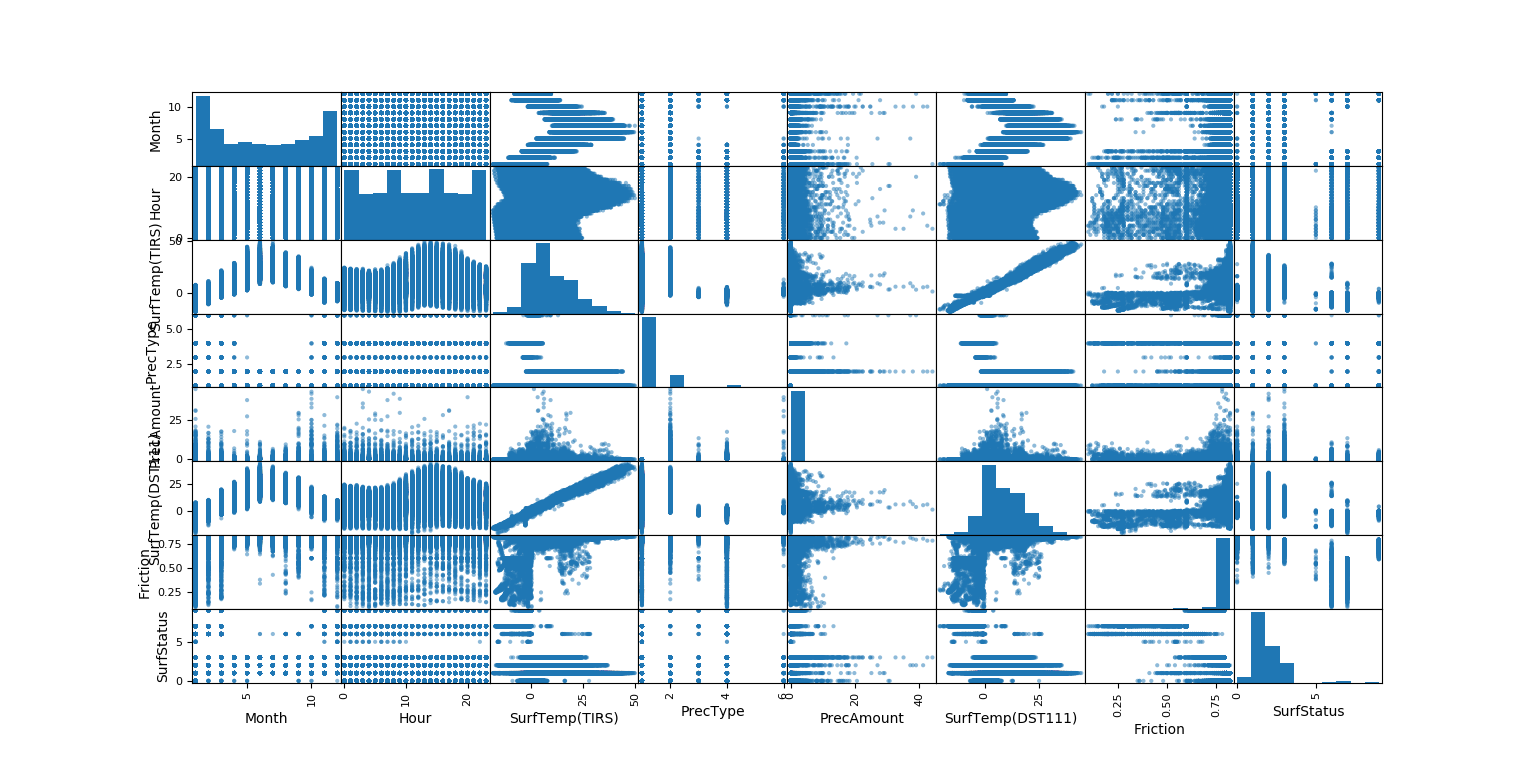
\includegraphics[width=1\textwidth]{media/correlations_featureengi.png}
	\caption{Correlations among the different features where month and hour are two new features that have replaced time. }
	\label{img:correlations_featureengi}
\end{figure}

	All that's left is to see the effects of the transformation. An experiment with Cross-validation regression spot-checking setup was used to study the effects of this new transformation. Table \ref{table:transformation_effect} shows the result.

	\begin{table}[H] %gör om med holdout
	\centering
	\caption{Experiment to see the effects of transforming the time feature is relevant to use as input feature. }
		\resizebox{\textwidth}{!}{%
		\begin{tabular}[6]{l | c | c | c |c | c}
    			Algorithm & MSE using neither time nor new features & MSE using time & MSE using hour and month & MSE using month & MSE using hour \\
    			\hline
			OLS & 1.23 & 1.22 & 1.22 & 1.22 & 1.21 \\
			CART & 1.21 & 1.84 & 1.77 & 1.34 & 1.39 \\
			kNN & 1.25 & 4.69 & 1.08 & 1.24 & 1.15 \\
			Backpropagation & 1.06 & 769096.72 & 1.30 & 1.06 & 1.08 \\
			Lasso & 1.25 & 1.24 & 1.23 & 1.24 & 1.23 \\
			Random forest & 1.13 & 1.26 & 1.01 & 1.02 & 1.12 \\
			\hline
			Total average & 1.19 & 128184.50 & 1.27 & 1.19 & 1.20
			\label{table:transformation_effect}
		\end{tabular}
		}
	\end{table}

	Performance is improved for all algorithms when the new features are used as a way to represent time rather than using the old feature. However, not using time, hour or month, seem to have slightly higher performance than using both hour and month, but similar to using either of them. Although little to no overall performance improvement was made, it was decided to use the transformed input features in the default features for spot checking. The reason is that this experiment is set up to test Track Ice Road Surface road temperature alone. The new features may prove more relevant with the other target features and different hyperparameter settings etc.


\subsection{Handling class imbalance} \label{sec:class_imbalance}
	From what is seen in \ref{img:histogram_surfstatus}, road surface status seem to suffer from class imbalance. But classifying road surface status is not a goal in this project. It is interesting to see if precipitation type suffers the same symptom since classifying that is a goal in this project. Figure \ref{img:correlations_featureengi} shows the distribution of precipitation type in the dataset. 
	
	\begin{figure}[H] 
	\centering
	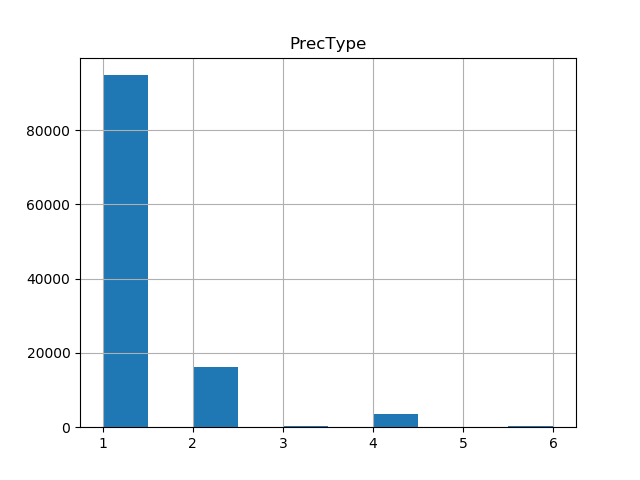
\includegraphics[width=1\textwidth]{media/histogram_prectype.png}
	\caption{Histogram showing the distribution of the different types of precipitation in the data (see \ref{table:occurences_prectype} to see what each code means).}
	\label{img:correlations_featureengi}
	\end{figure}

	The exact number of occurences and a translation of what each code means is shown in \ref{table:occurences_prectype}.

	\begin{table}[H]
	\centering
	\caption{Number of occurrences for different types of precipitation. }
		\begin{tabular}[3]{c | l | l}
    			Code & Precipitation type & no occurrences \\
    			\hline
			1 & no precipitation & 94825 \\
			2 & rain with $>= 0 \celsius$ air temperature & 16094 \\
			3 & rain with $< 0 \celsius$ air temperature & 266 \\
			4 & snow & 3677 \\
			6 & rain and snow mixed & 316 \\
			\label{table:occurences_prectype}
		\end{tabular}
	\end{table}

	From what can be seen in \ref{table:occurences_prectype}, precipitation also suffers a significant class imbalance. The biggest difference is between no precipitation and rain and snow mixed, the former appear $~300$ times more than that the latter.

	An experiment was carried out to see if the class imbalance problem can be mitigated by using random oversampling as oversampling technique (see \ref{sec:imbalanced_data_theory}. Random oversampling and Smote was tested in this experiment. Smote runs on the default settings as seen in \ref{WEBSITE:23}. Both random oversampling and Smote are compared to a scenario where oversampling is not used. All three scenarios run the holdout classification spot-checking setup with feature engineered features \ref{sec:exp_setups}. Holdout was used instead of $k$-fold in both scenarios since it proved cumbersome to integrate oversampling with $k$-fold, plus a confusion matrix can be obtained when the holdout method is used in Scikit-learn, which can make the results easier to interpret. 

	\begin{table}[H]
	\centering
	\caption{Results from not using any oversampling techniques. }
		\begin{tabular}[5]{l | c | c | c | c}
    			Algorithm & Accuracy & $\overline{Precision}$ & $\overline{Recall}$ & $\overline{F_1}$ \\
    			\hline
			LR & 0.81 & 0.24 & 0.21 & 0.21  \\
			kNN & 0.86 & 0.51 & 0.35 & 0.39  \\
			CART & 0.86 & 0.53 & 0.36 & 0.40 \\
			NB & 0.82 & 0.44 & 0.26 & 0.26  \\
			Backpropagation & 0.86 & 0.47 & 0.33 &  0.38  \\
			Random forest & 0.86 & 0.56 & 0.37 & 0.41  \\
			\hline
			Total average & 0.85 & 0.46 & 0.31 & 0.34
			\label{table:no_oversampling}
		\end{tabular}
	\end{table}

	\begin{table}[H]
	\centering
	\caption{Results from using random oversampling as oversampling technique.}
		\begin{tabular}[5]{l | c | c | c | c}
    			Algorithm & Accuracy & $\overline{Precision}$ & $\overline{Recall}$ & $\overline{F_1}$ \\
    			\hline
			LR & 0.48 & 0.33 & 0.55 & 0.31 \\
			kNN & 0.57 &  0.31 & 0.52 &  0.31 \\
			CART & 0.63 & 0.33 & 0.54 &  0.34 \\
			NB &  0.52 & 0.36 & 0.54 & 0.31 \\
			Backpropagation & 0.62 & 0.36 & 0.60 & 0.36 \\
			Random forest & 0.63 & 0.33 & 0.54 &  0.34 \\
			\hline
			Total average & 0.58 & 0.34 & 0.55 & 0.33 
			\label{table:random_oversampling}
		\end{tabular}
	\end{table}

	\begin{table}[H]
	\centering
	\caption{Results from using Smote as oversampling technique.}
		\begin{tabular}[5]{l | c | c | c | c}
    			Algorithm & Accuracy & $\overline{Precision}$ & $\overline{Recall}$ & $\overline{F_1}$ \\
    			\hline
			LR & 0.48 & 0.33 & 0.56 & 0.31 \\
			kNN & 0.68 &  0.31 & 0.47 &  0.34 \\
			CART & 0.72 & 0.33 & 0.48 &  0.35 \\
			NB &  0.53 & 0.36 & 0.53 & 0.31 \\
			Backpropagation & 0.62 & 0.37 & 0.60 & 0.36 \\
			Random forest & 0.72 & 0.33 & 0.49 &  0.36 \\
			\hline
			Total average & 0.63 & 0.34 & 0.52 & 0.33 
			\label{table:smote_oversampling}
		\end{tabular}
	\end{table}
	
	Table \ref{table:no_oversampling} and \ref{table:random_oversampling} shows the effects of using random oversampling versus no oversampling: total average accuracy and precision is reduced, total average recall is higher, and total average $F_1$ score is similar to the case when oversampling is not used. In the case of using Smote as oversampling technique as shown in \ref{table:smote_oversampling}, it proved to have similar effects of using random oversampling. Both precision and recall are important in this project when it comes to evaulating classification algorithm performance. Since no improvement was made on the collective score of precision and recall: $F_1$, and overall accuracy was reduced when either of the oversampling techniques were tested, oversampling was ruled out as a possible solution to handle imbalanced classes. 

	Since the multiclass classification problem is but one of four subtasks in this project, additional effort was not put in to investigate if the imbalanced dataset problem can be solved in other ways.